\documentclass[a4paper,12pt]{article} %style de document
\usepackage[utf8]{inputenc} %encodage des caractères
\usepackage[french]{babel} %paquet de langue français
\usepackage[T1]{fontenc} %encodage de la police
\usepackage[top=2cm,bottom=2cm,left=2cm,right=2cm]{geometry} %marges
\usepackage{graphicx} %affichage des images
\usepackage{url}
\usepackage{verbatim}


\begin{document} %début du document

%----------------------------------
%page de garde
%----------------------------------

\begin{titlepage}
	\begin{center}
		
		\huge{Compte-rendu du projet de TPA: le Sokoban}\\
		\vspace{2cm}
		
		%\includegraphics[scale=0.6]{Image du jeu}\\
		% mettre une image du jeu fini
		\medskip
		\vspace{2cm}
		DE OLIVEIRA Dylan\\
		GARCIA Romain \\
		NGUYEN Michael \\
		VINCIGUERRA Antoine\\
		\normalsize{\textit{ ~ L2 Informatique}}\\
		\Large{Année universitaire 2017-2018}\\
		\Large{Université de Caen Basse-Normandie}\\[1cm]
			
\end{center}
\end{titlepage}

\newpage

%----------------------------------
%sommaire
%----------------------------------

\begin{center}
\renewcommand{\contentsname}{Sommaire}
\tableofcontents
\end{center}


%----------------------------------
%Contenu du compte-rendu
%----------------------------------

\newpage

%----------------------------------
%Introduction du jeu 
%----------------------------------
\section{Introduction}
	\subsection{Pourquoi ce projet et que cela peut-il apporter au groupe  ?}
	Le projet en Travail Personnel Approfondi ou TPA nous permet de mettre en pratique nos connaissances sur la programmation orientée objet en langage Java.

\paragraph{}
	
	Il y a différentes choses que nous pouvons tirer de ce projet: d'abord, le travail en groupe, car lorsque l'on sera en entreprise, nous aurons à travailler avec en groupe. L'adaptabilité, la curiosité, acquérir du savoir ou des méthodes jamais vu en cours qui pourront être réutiliser dans le cadre d'un autre projet ou en entreprise.
	   
	\subsection{Le sujet}
	
	Les sujets possibles pour le projet étaient les suivant:
	\vspace{0.1cm}
	
\begin{itemize}
\item CoreWar
\item Sokoban
\item Editeur de sprite
\item Logiciel stéganographie
\item Le Castor Affairé
\item Lecteur de musique augmenté
\end{itemize}
\paragraph{}		

	Après réflexion en groupe, nous avons décidé de faire le sokoban car ce projet plaisait à tout le groupe, il permet de mettre en œuvre nos connaissances en Java mais aussi de pouvoir aller plus loin pour approfondir nos connaissances en la matière en ayant une programmation orienté objet au maximum en suivant le modèle MVC.
	
	\subsection{Le sokoban}
	Voici une présentation rapide de l'histoire du sokoban.
	
	\subsubsection{Son histoire}
	Le jeu original a été écrit par Hiroyuki Imabayashi et comportait 50 niveaux. Il remporte en 1980 un concours de jeu vidéo pour ordinateur. Plus tard Hiroyuki Imabayashi est devenu président de la compagnie japonaise Thinking Rabbit Inc. qui détient aujourd'hui les droits sur le jeu depuis 1982.
	
\paragraph{}

	Aujourd'hui, il existe de multiples jeux dérivés de ce jeu, par exemple Boxworld, une variante fonctionnant sous Windows et incluant 100 niveaux. Microsoft proposait ce jeu sous le nom de « Pousse Bloc ». Comme les règles sont simples, le jeu est facile à programmer. Plusieurs versions ont été écrites en JavaScript ; il est ainsi possible de jouer en ligne avec un navigateur web. Il existe des logiciels proposant un affichage 3D (le principe du jeu reste en 2D, comme certains jeux d'échecs 3D).
	
\paragraph{}

	Certains jeux (par exemple Push Crate) mettent en place de nouveaux éléments de gameplay pour Sokoban tels que des trous, des téléportations, ... [\textit{Source: Wikipédia}]

\newpage

%----------------------------------
%Partie montrant les classes du jeu
%----------------------------------

\section{Le jeu}

	\subsection{Présentation du jeu}
	
	\subsubsection{Ses règles}
	En tant que gardien d'entrepôt (divisé en cases carrées), le joueur doit ranger des caisses sur des cases cibles. Il peut se déplacer dans les quatre directions, et pousser (mais pas tirer) une seule caisse à la fois. Une fois toutes les caisses rangées (c'est parfois un vrai casse-tête), le niveau est réussi et le joueur passe au niveau suivant, plus difficile en général. L'idéal est de réussir avec le moins de coups possibles (déplacements et poussées). [\textit{Source: Wikipédia}]
	
	\subsubsection{Le cahier des charges fonctionnel}
	
	Le cahier des charges nous a permis de classer par priorité les différentes fonctionnalités, avec ses contraintes, pour la réalisation de notre Sokoban allant de la plus primordiale à la plus gadget. Mais il ne sert pas qu'à classer les fonctionnalités mais aussi nous indiquer la charge de travail que nous auront à réaliser.
	
	\begin{center}
	\begin{tabular}{| l | c | r |}
	\hline
	F1 & \textbf{Fonction} & \textbf{Être jouable par un humain} \\ \hline %rouge
	C1.1 & Contrainte & Avoir une interface \\ \hline
	C1.2 & Contrainte & Permettre au joueur de se déplacer \\ \hline
	C1.3 & Contrainte (bonus) & Tutoriel des mouvements en début de partie \\ \hline
	F2 & \textbf{Fonction} & \textbf{Avoir plusieurs niveaux de jeu} \\ \hline
	C2.1 & Contrainte & Importer des niveaux depuis des fichiers \\ \hline
	C2.2 & Contrainte & Respecter un format de donnée spécifique (.xsb, .sok ou .stb) \\ \hline
	C2.3 & Contrainte & Intégrer des objectifs de fin (résolvable) \\ \hline
	F3 & \textbf{Fonction} & \textbf{Avoir un système de résolution automatique} \\ \hline %rouge
	C3.1 & Contrainte & Intégrer une intelligence artificielle de résolution \\ \hline
	F4 & \textbf{Fonction} & \textbf{Permettre de faire jouer humain et ordinateur en parallèle} \\ \hline
	C4.1 & Contrainte & Rendre \textit{anytime}* l'algorithme de l'IA \\ \hline
	F5 & \textbf{Fonction} & \textbf{Intégrer une interface graphique} \\ \hline
	F6 & \textbf{Fonction (bonus)} & \textbf{Intégration d'un système de score} \\ \hline %rouge
	C6.1 & Contrainte (bonus) & Nombre de mouvements \\ \hline
	C6.2 & Contrainte (bonus) & Durée de la partie \\ \hline
	C6.3 & Contrainte (bonus) & Nombre d'essais \\ \hline
	F7 & \textbf{Fonction (bonus)} & \textbf{Classement en fonction du score} \\ \hline
	C7.1 & Contrainte (bonus) & Stockage des cores dans un fichier \\ \hline
	C7.2 & Contrainte (bonus) & Gestion de joueurs multiples(nom) \\ \hline
	\hline
	\end{tabular}
	\vspace{0.01cm}
	\textit{* l’intelligence artificielle est obligée de jouer dès que l'humain fait un mouvement}
	\end{center}
			
\newpage %Pour une meilleur lisibilité
	\subsubsection{Les différentes contraintes à respecter}
	
	A l'aide du cahier des charges et des règles du jeu, nous avons différentes contraintes à respecter pour qu'il soit à la fois jouable et corresponde à notre vision. De ce fait, nos contraintes sont à ajouter avec les règles de bases du jeu citées plutôt dans le rapport.
	
\paragraph{}

Les contraintes de base du jeu:
\vspace{0.2cm}
\begin{itemize}
\item Le joueur ne peut pas tirer une caisse, il ne peut que la pousser et une seule à la fois
\item Le joueur doit mettre les caisses sur les cases d'arrivée pour passer au niveau suivant
\item Le personnage du joueur ou les caisses ne doivent pas passer à travers les murs ou d'autres caisses
\end{itemize}
\paragraph{}

Les contraintes qui nous sont imposés:
\vspace{0.2cm}
\begin{itemize}
\item Avoir un tutoriel pour les mouvements
\item Intégrer une résolution automatique du niveau par une IA
\item Intégrer une IA
\item Permettre au joueur de jouer contre l'IA
\item Afficher le nombre de mouvements, durée de la partie, le nombre d'essais
\item Stocker les scores
\item Gérer plusieurs joueurs
\end{itemize}
	\subsubsection{Diagramme UML}
	La figure ci-dessous est le diagramme UML de nos différentes classes qui seront utilisé pour la réalisation de notre Sokoban:\\
	% mettre le Diagramme ici
	\begin{center}
	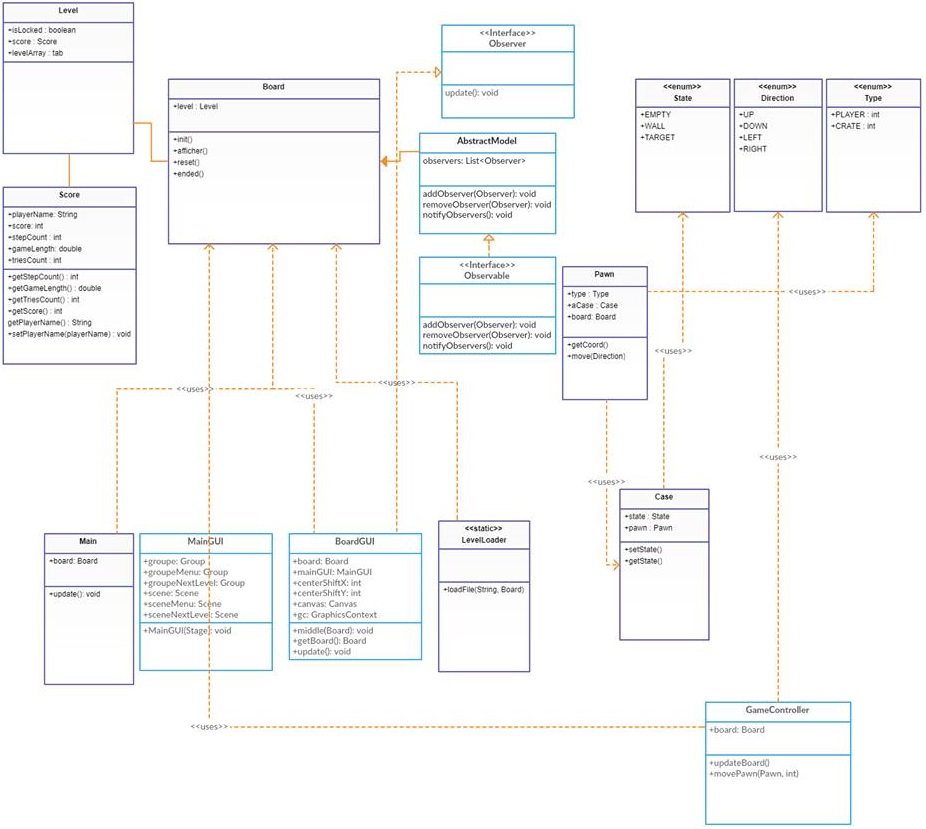
\includegraphics[scale=0.56]{uml.png}
	\end{center}
	Nous l'avons établi à la suite du cahier des charges et il nous a servi de support tout au long du projet.
	
	\paragraph{}
	
	\subsection{Présentation des différents packages}
	
		\subsubsection{Model}
		Dans le modèle MVC, le package Model est le package le plus riche, c'est la base de l'application. Il contient tous les objets et les méthodes de celles-ci.
		
		\subsubsection{View}
		Le package View n'est qu'enfaite que l'interface humain machine.
	
		\subsubsection{Controller}
		Le Controller permet de relier les deux packages précédents, le Model et la View. Il reçoit des informations du package View, vérifie si l'action ou les actions demandées sont faisables et envoie les directives au package Model afin d'appliquer les actions et d'actualiser la View. 

\newpage

%----------------------------------
% Eléments techniques
%----------------------------------

\section{Éléments techniques}
	
	\subsection{Algorithme}
		\subsubsection{Les déplacements}
		Dans cette partie nous allons détailler des déplacements, leur fonctionnement et pourquoi nous avons choisi de les faire ainsi.\\
		Les mouvements sont gérés par le GameController qui prend en paramètres un pion et une direction (UP, DOWN, LEFT, RIGHT) qui est issue d'une énumeration. La méthode move(Pawn pawn, Direction direction) est simplement composée d'un switch et de quatre cas, pour chaque direction on vérifie si la case suivant le pion n'est pas un mur, si ce n'est pas un mur on vérifie si c'est une boîte et enfin on verifie s'il y a un obstacle derrière celle-ci, on finit en déplaçant le pion.\\
		
%Intégrer pseudo-code
		
		\subsubsection{L'IA}
		Dans le cadre du projet, il nous était demandé de créer une IA s'inspirant de A* (A star) qui est un algorithme de recherche de chemin dans un graphe entre un noeud initial et un noeud final tous deux donnés. Il a été crée pour que la première solution trouvée soit l'une des meilleures.\\
		Notre IA commence par sélectionner la caisse la proche du joueur et la cible la plus proche de la caisse. Ensuite on créer le chemin partant de la caisse sélectionnée ultérieurement et la cible la plus proche de celle-ci, puis on construit une liste de chemin possible. Pour chaque déplacement, si la direction change, on replace le joueur au bon endroit autour de la caisse afin de la pousser dans la bonne direction. Pour finir on créer la liste des déplacements nécessaires afin de positioner le pion faisant face à la caisse dans la bonne direction.\\
	
%Intégrer pseudo-code

	\subsection{L'interface graphique}
		\subsubsection{JavaFX}
		\begin{center}
		
\includegraphics[scale=0.3]{javafx_logo.jpg}
		\end{center}
		JavaFX est une API Java, c'est une technologie créée par Sun Microsystems (maintenant Oracle) et qui est devenu la bibliothèque de création d'interface graphique officielle du langage Java dû à l'abandon de développement de son prédécesseur Swing. JavaFX permet de développer toutes sortes d'application (mobiles, web) avec de nombreux outils pour le graphisme en 2D et 3D, le Web, l'audio ou même les vidéos. Il est désormais intégré au JDK SE, donc il n'y a pas besoin de télécharger et d'installer quoique ce soit. Il existe de nombreux compléments à JavaFX comme par exemple ControlsFX qui permet de réaliser des UI de meilleure qualité.
		
		\subsubsection{Pourquoi JavaFX?}
		Lorsque nous avons établi le cahier des charges, nous envisagions d'utiliser Swing ou AWT afin de réaliser l'interface graphique. Cependant lors d'une réunion de travail, grâce aux connaissances de l'un des membres nous avons appris que, les deux bibliothèques citées précédemment n'étaient plus en developpement, nous avons donc décidé d'utiliser JavaFX qui comme présenté plus tôt est le langage officielle de créaion d'interface graphique du langage Java.
	
\newpage

%----------------------------------
% Expérimentation 
%----------------------------------

\section{Expérimentation sur le jeu}
	\subsection{Test du jeu sans l'interface graphique}
	
	\subsubsection{Test des règles du jeu}
	Le but de cette expérience est de vérifier si les règles du jeu sont bien implémentées et qu'aucun problèmes n'apparaissent. Tout d'abord, nous avons vérifier que les mouvements se faisaient sans problèmes.
	\paragraph{}
	
	Ce fut le premier test que nous avons fait, tout d'abord en ligne de commande dans la console, puis avec le GUI. Commençons par les déplacements simples du personnage dans son environnement.
	\paragraph{}
	\begin{center}
	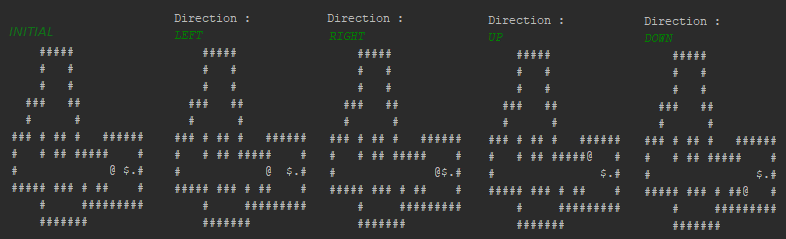
\includegraphics[scale=0.65]{Tests-mouvements-console.png}
	\end{center}
	%mettre une image du personnage qui se déplace sur le bord
	%mettre un titre à l'image
		
	Le personnage n'a aucun souci pour se déplacer. Ensuite nous allons tester le déplacement d'une caisse.
	\paragraph{}
	\begin{center}
	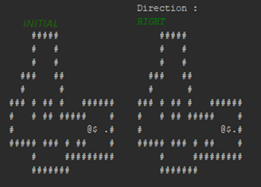
\includegraphics[scale=1]{Tests-mouvements-caisse-console.png}
	\end{center}
	%mettre une image du personnage poussant une caisse
	%mettre un titre à l'image
	
	Pour finir, nous allons tester la fin de partie.
	\paragraph{}
	\begin{center}
	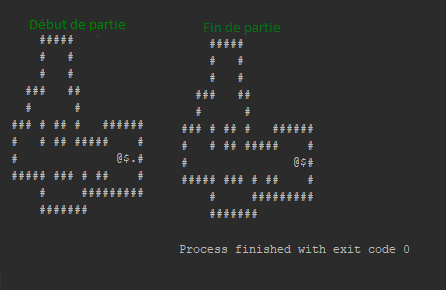
\includegraphics[scale=0.7]{Tests-partie-finie-console.png}
	\end{center}
	%mettre une image du personnage poussant une caisse contre un mur et le personne essayant de passer à travers un mur
	%mettre un titre à l'image
	
	\subsubsection{Test des règles du jeu}
	
	\subsection{Test du jeu avec l'interface graphique}
	Comme dans la partie précédente, nous allons refaire nos tests pour vérifier s'il n'y a pas de problèmes.
	\paragraph{}
	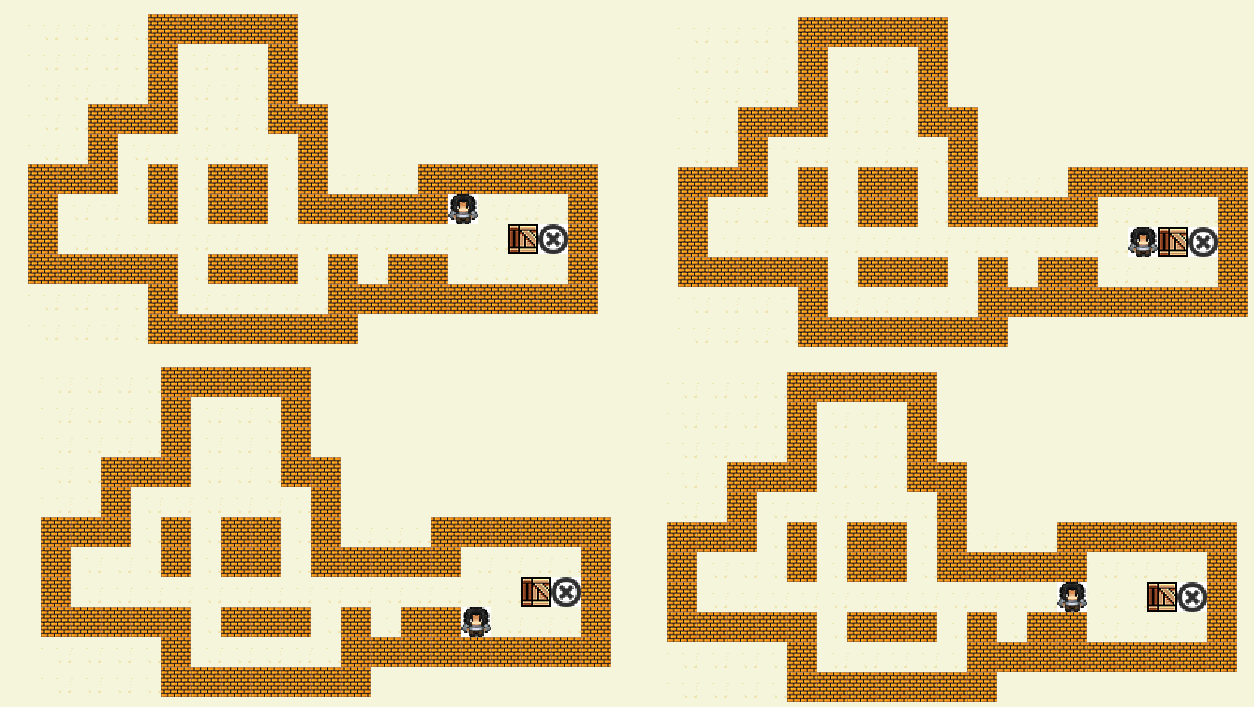
\includegraphics[scale=0.5]{Tests-mouvements-GUI.png}
	%mettre une image de plusieurs commandes de déplacement
	%mettre un titre à l'image
	%ajout d'explication de pourquoi faire ce test
	Nous n'avons pas rencontré de problèmes au cours de ce test, les fonctions de déplacements simple sont donc fonctionnelles.\\
	
	Ensuite, nous avons testé si le fait de pousser une caisse ne générait pas d'erreur.\\
	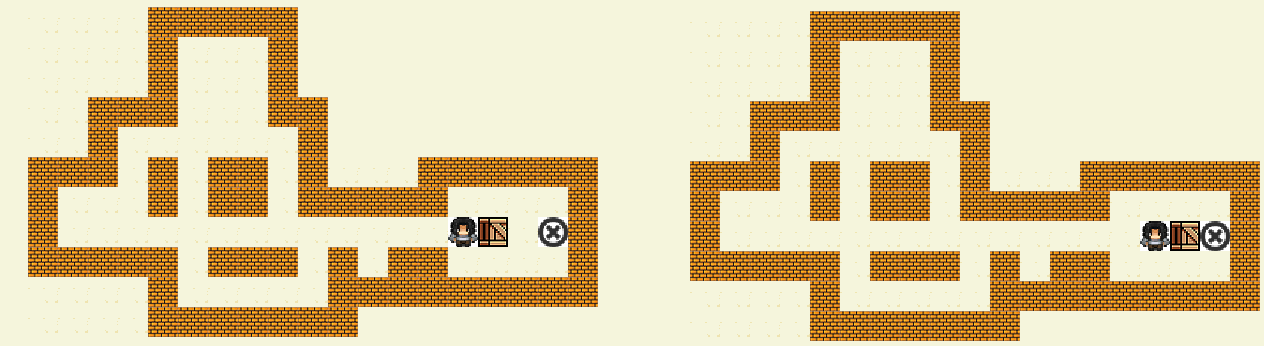
\includegraphics[scale=0.5]{Tests-mouvements-caisse-GUI.png}
	\paragraph{}
	%mettre une image du personnage poussant une caisse
	%mettre un titre à l'image	
	%ajout d'explication de pourquoi faire ce test
	
	\paragraph{}
	%mettre une image du personnage poussant une caisse contre un mur et le personnage essayant de passer à travers un mur
	%mettre un titre à l'image
	%ajout d'explication de pourquoi faire ce test
	
	En conclusion, le jeu sous le GUI a passé nos tests sans difficultés.
	
	\subsubsection{Expérimentation sur l'IA}

	\subsection{Performance}
	En ce qui concerne les performances, on a essayé d'optimiser au maximum l'application. En idle, on est sur 0\% d'utilisation du processeur (sur un processeur Intel Core i5-6300HQ Quad Core @2.3GHz). Lors de la génération de l'application on monte au maximum à 30-34\% d'utilisation, puis on retombe à 3\% en idle. Lors de déplacement simple (joeur ou caisse) on monte à 6\%. Et enfin lors de la resolution du niveau par l'IA on monte à  42\% d'utilisation.\\
	Pour les tests, nous avons résolu le niveau 1 du sokoban en 54 coups en l'espace de 10 secondes 3, de l'autre côté l'IA résolu le niveau en 56 coups en l'espace de 236ms. Pour le niveau 2 qui est un peu plus compliqué, on le résolu en 278 coups en l'espace de 57 secondes, l'IA quant à lui le résolu en 227 coups et 5 secondes. Les test ont étés réalisé en faisant la moyenne sur 20 parties et en arrondissant à l'entier supérieur.\\
	
	%mettre le taux de consommation du processeur
	%Faire des comparatifs entre les joueurs et l'IA
	
\newpage
%----------------------------------
% Conclusion
%----------------------------------

\begin{center}
\section{Conclusion}
\end{center}

	\subsection{Récapitulatif des fonctionnalités principales}
	A l'heure actuelle, nous avons réaliser les fonctions du cahier des charges: La fonction 1, qui est de rendre le jeu jouable par un humain, ainsi que les différentes contraintes (sauf celle bonus). La fonction 2 et ses contraintes visant à avoir plusieurs niveaux, de pouvoir en importer, de respecter le format donnée et d'intégrer des objectifs de fin. La fonction 3La fonction 5 étant la fait d'avoir une interface graphique.
	\subsection{Proposition d'améliorations}
	Le projet pourra être amélioré en changeant l'interface d'utilisateur, en ajoutant des fonctionnalités tels que le choix de personnage, la sauvegarde de score, un système de classement. Ces amélioration étaient présente lorsque nous avons établi le cahier des charges mais les problèmes techniques rencontrés ont étés plus longs à résoudre que prévu. De plus, anytime n'est pas disponible dans cette version car nous n'avons pas réussi à résoudre un problème lié à l'implémentation de deux board simultanément, elle sera peut-être disponible dans une prochaine version. 

\newpage

%----------------------------------
% Annexe  
%----------------------------------

\begin{center}
\section{Annexe}
\end{center}
Voici les différentes documentations utilisées pour la création de notre Sokoban:
\begin{itemize}
\item Documentation JavaFX
\item Documentation sur l'algorithme A*
\end{itemize}
\paragraph{}

Les différentes sources pour notre documentation:
\begin{itemize}
\item Openclassroom
\item Wikipédia
\item Oracle
\end{itemize}
\begin{center}
\section{Remerciement}
\end{center}

Nous souhaitons remercier particulièrement : 
\begin{itemize}
\item Monsieur VALLEE Thibaut, Professeur d'Expression et Communication
\item Monsieur BADAOUI Mohamad, Professeur du Complément de POO
\item Monsieur CABANA Antoine, Professeur de Travail Personnel Approfondi
\end{itemize}
Pour tout le savoir, les exercices de mise en pratique de ce savoir et leur aide pendant la réalisation de notre projet.


\end{document}
